%% chapters/chapter_1.tex
%%
%% Copyright 2017 Evandro Coan
%% Copyright 2012-2014 by abnTeX2 group at http://abntex2.googlecode.com/
%%
%% This work may be distributed and/or modified under the
%% conditions of the LaTeX Project Public License, either version 1.3
%% of this license or (at your option) any later version.
%% The latest version of this license is in
%%   http://www.latex-project.org/lppl.txt
%% and version 1.3 or later is part of all distributions of LaTeX
%% version 2005/12/01 or later.
%%
%% This work has the LPPL maintenance status `maintained'.
%%
%% The Current Maintainer of this work is the Evandro Coan.
%%
%% The last Maintainer of this work was the abnTeX2 team, led
%% by Lauro César Araujo. Further information are available on
%% https://www.abntex.net.br/
%%
%% This work consists of a bunch of files. But originally there were 2 files
%% which are renamed as follows:
%% Deleted the `abntex2-modelo-img-marca.pdf`
%% Renamed the `abntex2-modelo-include-comandos.tex, v-1.9.2 laurocesar` to `chapters/chapter_1.tex`
%%
% ---
% Este capítulo, utilizado por diferentes exemplos do abnTeX2, ilustra o uso de
% comandos do abnTeX2 e de LaTeX.
% ---

% The \phantomsection command is needed to create a link to a place in the document that is not a
% figure, equation, table, section, subsection, chapter, etc.
% https://tex.stackexchange.com/questions/44088/when-do-i-need-to-invoke-phantomsection
\phantomsection

% https://tex.stackexchange.com/questions/5076/is-it-possible-to-keep-my-translation-together-with-original-text
\chapter[\lang{Abbreviation for the Table of Contents}{Abreviação para o Sumário}]
{
    \lang
    {Long title to present in the chapter, Axioms, Theorems, Postulates, corollaries, lemmas}
    {Longo título apresentar no capítulo, Axiomas, Teoremas, Postulados, corolários, lemas}
}

\label{cap_exemplos}


\begin{flushright}
    \englishword{\showfont}
\end{flushright}

% Why latex is letting my text goes out of the screen?
% https://tex.stackexchange.com/questions/386762/why-latex-is-letting-my-text-goes-out-of-the-screen
\sloppy
\textbf{textbf: \englishword{\showfont}}
\fussy



\section{Axiomas ou postulados}

Na lógica tradicional, um axioma ou postulado é uma sentença ou proposição que não é provada ou demonstrada e é considerada como óbvia ou como um consenso inicial necessário para a construção ou aceitação de uma teoria. Por essa razão, é aceito como verdade e serve como ponto inicial para dedução e inferências de outras verdades (dependentes de teoria). -- \showfont


Na matemática, um axioma é uma hipótese inicial de qual outros enunciados são logicamente derivados. Pode ser uma sentença, uma proposição, um enunciado ou uma regra que permite a construção de um sistema formal. Diferentemente de teoremas, axiomas não podem ser derivados por princípios de dedução e nem são demonstráveis por derivações formais, simplesmente porque eles são hipóteses iniciais. Isto é, não há mais nada a partir do que eles seguem logicamente (em caso contrário eles seriam chamados teoremas). Em muitos contextos, "axioma", "postulado" e "hipótese" são usados como sinônimos. -- \showfont


\begin{axioma}[Axioma de Igualdade -- \showfont]
Supondo $\mathfrak{L}$, uma linguagem de primeira ordem. para cada variável $x$, a fórmula $x = x$ é universalmente válida. -- \showfont
\end{axioma}


\begin{postulado}[Postulado de Igualdade -- \showfont]
    Supondo $\mathfrak{L}$, uma linguagem de primeira ordem. para cada variável $x$, a fórmula $x = x$ é universalmente válida. -- \showfont
\end{postulado}


\section{Teorema}

Na matemática, um teorema é uma afirmação que pode ser provada como verdadeira através de outras afirmações já demonstradas, como outros teoremas, juntamente com afirmações anteriormente aceitas, como axiomas. Prova é o processo de mostrar que um teorema está correto. O termo teorema foi introduzido por Euclides, em Elementos, para significar "afirmação que pode ser provada". Em grego, originalmente significava "espetáculo" ou "festa". Atualmente, é mais comum deixar o termo "teorema" apenas para certas afirmações que podem ser provadas e de grande "importância matemática", o que torna a definição um tanto subjetiva.

\begin{teorema}[Teorema de Pitágoras -- \showfont]
    Em qualquer triângulo retângulo, o quadrado do comprimento da hipotenusa é igual à soma dos quadrados dos comprimentos dos catetos -- \showfont.
\end{teorema}


\begin{proposicao}
Em qualquer proposição a hipótese é considerada verdadeira. -- \showfont
\end{proposicao}


\subsection{Terminologia}

Usualmente deixa-se o termo ``teorema'' apenas para as afirmações que podem ser provadas de grande importância. Assim, são dados outros nomes para os outros tipos dessas afirmações -- \showfont:

\begin{description}
    \item[Proposição:] Uma Proposição é uma sentença não associada a algum outro teorema, de simples prova e de importância matemática menor -- \showfont.
    \item[Lema:] Um Lema é um ``pré-teorema'', um teorema que serve para ajudar na prova de outro teorema maior. A distinção entre teoremas e lemas é um tanto quanto arbitrária, uma vez que grandes resultados são usados para provar outros. Por exemplo, o Lema de Gauss e o Lema de Zorn são muito interessantes de per se, e muitos autores os denominam de Lemas, mesmo que não os usem para provar alguma outra coisa. -- \showfont
    \item[Corolário:] Um Corolário é uma consequência direta de outro teorema ou de uma definição, muitas vezes tendo suas demonstrações omitidas, por serem simples. -- \showfont
\end{description}


\begin{corolario}
    Em qualquer triângulo retângulo, a hipotenusa é maior que qualquer um dos catetos, mas menor que a soma deles. -- \showfont
\end{corolario}

Alguns outros termos também são usados, por mais que raros e com definição menos rigorosa, basicamente sendo usadas quando não se quer usar a a palavra ``teorema'' -- \showfont:

Regra.
Lei, que também pode se referir a axiomas, regras de dedução e a distribuições de Probabilidade.
Princípio.
Algoritmo (como em Algoritmo da Divisão), muito raro e diferente do conceito com o mesmo nome que é um dos estudos centrais da Ciência da Computação.
Paradoxo, usado quando a afirmação vai aparentemente de encontro com alguma outra verdade ou com alguma noção intuitiva. Entretanto, tal termo também pode ser usado para afirmações falsas que aparentem ser verdadeiras em um primeiro momento. -- \showfont

Alguns teoremas continuam a ser chamados de Conjecturas logo após serem provados (por exemplo, a Conjectura de Poincaré). O termo conjectura é usado para afirmações que não se sabe se são verdadeiras, e que acredita-se que são verdadeiras, mas nunca ninguém conseguiu prová-las nem negá-las (às vezes conjecturas são chamadas de hipóteses (como em Hipótese de Riemann), obviamente, num sentido diferente do aqui já descrito). -- \showfont


\subsection{Conjectura ou hipótese}

Uma conjectura é uma ideia, fórmula ou frase, a qual não foi provada ser verdadeira, baseada em suposições ou ideias com fundamento não verificado. As conjecturas utilizadas como prova de resultados matemáticos recebem o nome de hipóteses. -- \showfont



\begin{conjectura}[Conjectura dos primos gêmeos -- \showfont]
Existem infinitos números primos gêmeos. -- \showfont
\end{conjectura}

Um par de primos é chamado de primos gêmeos se eles são dois números primos $p$, $q$ tais que $q = p + 2$. -- \showfont



\subsection{Lema}

    Na Matemática, um lema é um teorema que é usado como um passo intermediário para atingir um resultado maior, provado em outro teorema. Normalmente o lema tem pouca serventia além de servir ao propósito do teorema que o utiliza, mas isto não é uma regra, e a classificação entre lemas e teoremas é arbitrária\footnote{Wikipédia -- \showfont} -- \showfont.



% https://tex.stackexchange.com/questions/20987/changing-babel-package-inside-a-single-chapter
\begin{otherlanguage*}{english}

\begin{lema}
    Given two line segments whose lengths are $a$ and $b$ respectively there is a
    real number $r$ such that $b=ra$. -- \showfont
\end{lema}



Unnumbered theorem-like environments are also possible -- \showfont.

\begin{observacao}
    This statement is true, I guess. -- \showfont
\end{observacao}

And the next is a somewhat informal definition. -- \showfont


\begin{definicao}[Fibration -- \showfont]
    A fibration is a mapping between two topological spaces that has the homotopy lifting property for every space $X$. -- \showfont
\end{definicao}

\begin{exemplo}[Fibration -- \showfont]
    A fibration is a mapping between two topological spaces that has the homotopy lifting property for every space $X$. -- \showfont
\end{exemplo}


\begin{exercicio}
    Este é um exercício -- \showfont

\end{exercicio}


\begin{exercicio}
    Mais um exercício para vocês... -- \showfont

\end{exercicio}


\begin{condicao}[Fibration -- \showfont]
    A fibration is a mapping between two topological spaces that has the homotopy lifting property for every space $X$. -- \showfont
\end{condicao}
Theorem styles

\begin{description}
    \item[definition] boldface title, romand body. Commonly used in definitions, conditions, problems and examples. -- \showfont
\item[plain] boldface title, italicized body. Commonly used in theorems, lemmas, corollaries, propositions and conjectures.
\item[remark] italicized title, romman body. Commonly used in remarks, notes, annotations, claims, cases, acknowledgments and conclusions.
\end{description}

\end{otherlanguage*}



\section{Rotação de equações}

trecho de código para rotacionar e reduzir a fonte de equações. -- \showfont

\begin{verbatim}
\begin{sideways}%
  \parbox{1\textheight}{%
      \begin{tiny}
          \begin{equation}

          \end{equation}
      \end{tiny}}
\end{sideways}
\end{verbatim}


Segue um exemplo de rotação de páginas -- \showfont: \newpage

\begin{sideways}%
    \parbox{1\textheight}{%
        \begin{tiny}
\begin{equation}
\left[ {{L_{sr}}} \right] = \left[ {\begin{array}{*{20}{c}}
    {\cos \left( \theta  \right)}&{\cos \left( {\theta  - 8\alpha } \right)}&{\cos \left( {\theta  - 7\alpha } \right)}&{\cos \left( {\theta  - 6\alpha } \right)}&{\cos \left( {\theta  - 5\alpha } \right)}&{\cos \left( {\theta  - 4\alpha } \right)}&{\cos \left( {\theta  - 3\alpha } \right)}&{\cos \left( {\theta  - 2\alpha } \right)}&{\cos \left( {\theta  - \alpha } \right)}\\
    {\cos \left( {\theta  - \alpha } \right)}&{\cos \left( \theta  \right)}&{\cos \left( {\theta  - 8\alpha } \right)}&{\cos \left( {\theta  - 7\alpha } \right)}&{\cos \left( {\theta  - 6\alpha } \right)}&{\cos \left( {\theta  - 5\alpha } \right)}&{\cos \left( {\theta  - 4\alpha } \right)}&{\cos \left( {\theta  - 3\alpha } \right)}&{\cos \left( {\theta  - 2\alpha } \right)}\\
    {\cos \left( {\theta  - 2\alpha } \right)}&{\cos \left( {\theta  - \alpha } \right)}&{\cos \left( \theta  \right)}&{\cos \left( {\theta  - 8\alpha } \right)}&{\cos \left( {\theta  - 7\alpha } \right)}&{\cos \left( {\theta  - 6\alpha } \right)}&{\cos \left( {\theta  - 5\alpha } \right)}&{\cos \left( {\theta  - 4\alpha } \right)}&{\cos \left( {\theta  - 3\alpha } \right)}\\
    {\cos \left( {\theta  - 3\alpha } \right)}&{\cos \left( {\theta  - 2\alpha } \right)}&{\cos \left( {\theta  - \alpha } \right)}&{\cos \left( \theta  \right)}&{\cos \left( {\theta  - 8\alpha } \right)}&{\cos \left( {\theta  - 7\alpha } \right)}&{\cos \left( {\theta  - 6\alpha } \right)}&{\cos \left( {\theta  - 5\alpha } \right)}&{\cos \left( {\theta  - 4\alpha } \right)}\\
    {\cos \left( {\theta  - 4\alpha } \right)}&{\cos \left( {\theta  - 3\alpha } \right)}&{\cos \left( {\theta  - 2\alpha } \right)}&{\cos \left( {\theta  - \alpha } \right)}&{\cos \left( \theta  \right)}&{\cos \left( {\theta  - 8\alpha } \right)}&{\cos \left( {\theta  - 7\alpha } \right)}&{\cos \left( {\theta  - 6\alpha } \right)}&{\cos \left( {\theta  - 5\alpha } \right)}\\
    {\cos \left( {\theta  - 5\alpha } \right)}&{\cos \left( {\theta  - 4\alpha } \right)}&{\cos \left( {\theta  - 3\alpha } \right)}&{\cos \left( {\theta  - 2\alpha } \right)}&{\cos \left( {\theta  - \alpha } \right)}&{\cos \left( \theta  \right)}&{\cos \left( {\theta  - 8\alpha } \right)}&{\cos \left( {\theta  - 7\alpha } \right)}&{\cos \left( {\theta  - 6\alpha } \right)}\\
    {\cos \left( {\theta  - 6\alpha } \right)}&{\cos \left( {\theta  - 5\alpha } \right)}&{\cos \left( {\theta  - 4\alpha } \right)}&{\cos \left( {\theta  - 3\alpha } \right)}&{\cos \left( {\theta  - 2\alpha } \right)}&{\cos \left( {\theta  - \alpha } \right)}&{\cos \left( \theta  \right)}&{\cos \left( {\theta  - 8\alpha } \right)}&{\cos \left( {\theta  - 7\alpha } \right)}\\
    {\cos \left( {\theta  - 7\alpha } \right)}&{\cos \left( {\theta  - 6\alpha } \right)}&{\cos \left( {\theta  - 5\alpha } \right)}&{\cos \left( {\theta  - 4\alpha } \right)}&{\cos \left( {\theta  - 3\alpha } \right)}&{\cos \left( {\theta  - 2\alpha } \right)}&{\cos \left( {\theta  - \alpha } \right)}&{\cos \left( \theta  \right)}&{\cos \left( {\theta  - 8\alpha } \right)}\\
    {\cos \left( {\theta  - 8\alpha } \right)}&{\cos \left( {\theta  - 7\alpha } \right)}&{\cos \left( {\theta  - 6\alpha } \right)}&{\cos \left( {\theta  - 5\alpha } \right)}&{\cos \left( {\theta  - 4\alpha } \right)}&{\cos \left( {\theta  - 3\alpha } \right)}&{\cos \left( {\theta  - 2\alpha } \right)}&{\cos \left( {\theta  - \alpha } \right)}&{\cos \left( \theta  \right)}
    \end{array}} \right]
\end{equation}
\end{tiny}
}
\end{sideways}


\begin{landscape}

Outra forma é utilizar o pacote pdflscape -- \showfont

% https://tex.stackexchange.com/questions/60453/reducing-font-size-in-equation
\tiny -- \showfont
\begin{equation}
\left[ {{L_{sr}}} \right] = \left[ {\begin{array}{*{20}{c}}
    {\cos \left( \theta  \right)}&{\cos \left( {\theta  - 8\alpha } \right)}&{\cos \left( {\theta  - 7\alpha } \right)}&{\cos \left( {\theta  - 6\alpha } \right)}&{\cos \left( {\theta  - 5\alpha } \right)}&{\cos \left( {\theta  - 4\alpha } \right)}&{\cos \left( {\theta  - 3\alpha } \right)}&{\cos \left( {\theta  - 2\alpha } \right)}&{\cos \left( {\theta  - \alpha } \right)}\\
    {\cos \left( {\theta  - \alpha } \right)}&{\cos \left( \theta  \right)}&{\cos \left( {\theta  - 8\alpha } \right)}&{\cos \left( {\theta  - 7\alpha } \right)}&{\cos \left( {\theta  - 6\alpha } \right)}&{\cos \left( {\theta  - 5\alpha } \right)}&{\cos \left( {\theta  - 4\alpha } \right)}&{\cos \left( {\theta  - 3\alpha } \right)}&{\cos \left( {\theta  - 2\alpha } \right)}\\
    {\cos \left( {\theta  - 2\alpha } \right)}&{\cos \left( {\theta  - \alpha } \right)}&{\cos \left( \theta  \right)}&{\cos \left( {\theta  - 8\alpha } \right)}&{\cos \left( {\theta  - 7\alpha } \right)}&{\cos \left( {\theta  - 6\alpha } \right)}&{\cos \left( {\theta  - 5\alpha } \right)}&{\cos \left( {\theta  - 4\alpha } \right)}&{\cos \left( {\theta  - 3\alpha } \right)}\\
    {\cos \left( {\theta  - 3\alpha } \right)}&{\cos \left( {\theta  - 2\alpha } \right)}&{\cos \left( {\theta  - \alpha } \right)}&{\cos \left( \theta  \right)}&{\cos \left( {\theta  - 8\alpha } \right)}&{\cos \left( {\theta  - 7\alpha } \right)}&{\cos \left( {\theta  - 6\alpha } \right)}&{\cos \left( {\theta  - 5\alpha } \right)}&{\cos \left( {\theta  - 4\alpha } \right)}\\
    {\cos \left( {\theta  - 4\alpha } \right)}&{\cos \left( {\theta  - 3\alpha } \right)}&{\cos \left( {\theta  - 2\alpha } \right)}&{\cos \left( {\theta  - \alpha } \right)}&{\cos \left( \theta  \right)}&{\cos \left( {\theta  - 8\alpha } \right)}&{\cos \left( {\theta  - 7\alpha } \right)}&{\cos \left( {\theta  - 6\alpha } \right)}&{\cos \left( {\theta  - 5\alpha } \right)}\\
    {\cos \left( {\theta  - 5\alpha } \right)}&{\cos \left( {\theta  - 4\alpha } \right)}&{\cos \left( {\theta  - 3\alpha } \right)}&{\cos \left( {\theta  - 2\alpha } \right)}&{\cos \left( {\theta  - \alpha } \right)}&{\cos \left( \theta  \right)}&{\cos \left( {\theta  - 8\alpha } \right)}&{\cos \left( {\theta  - 7\alpha } \right)}&{\cos \left( {\theta  - 6\alpha } \right)}\\
    {\cos \left( {\theta  - 6\alpha } \right)}&{\cos \left( {\theta  - 5\alpha } \right)}&{\cos \left( {\theta  - 4\alpha } \right)}&{\cos \left( {\theta  - 3\alpha } \right)}&{\cos \left( {\theta  - 2\alpha } \right)}&{\cos \left( {\theta  - \alpha } \right)}&{\cos \left( \theta  \right)}&{\cos \left( {\theta  - 8\alpha } \right)}&{\cos \left( {\theta  - 7\alpha } \right)}\\
    {\cos \left( {\theta  - 7\alpha } \right)}&{\cos \left( {\theta  - 6\alpha } \right)}&{\cos \left( {\theta  - 5\alpha } \right)}&{\cos \left( {\theta  - 4\alpha } \right)}&{\cos \left( {\theta  - 3\alpha } \right)}&{\cos \left( {\theta  - 2\alpha } \right)}&{\cos \left( {\theta  - \alpha } \right)}&{\cos \left( \theta  \right)}&{\cos \left( {\theta  - 8\alpha } \right)}\\
    {\cos \left( {\theta  - 8\alpha } \right)}&{\cos \left( {\theta  - 7\alpha } \right)}&{\cos \left( {\theta  - 6\alpha } \right)}&{\cos \left( {\theta  - 5\alpha } \right)}&{\cos \left( {\theta  - 4\alpha } \right)}&{\cos \left( {\theta  - 3\alpha } \right)}&{\cos \left( {\theta  - 2\alpha } \right)}&{\cos \left( {\theta  - \alpha } \right)}&{\cos \left( \theta  \right)}
    \end{array}} \right]
\end{equation}
\normalsize

\end{landscape}


% ---
\section{Codificação dos arquivos: UTF8}
% ---

A codificação de todos os arquivos do \abnTeX{} é \texttt{UTF8}. É necessário que
você utilize a mesma codificação nos documentos que escrever, inclusive nos
arquivos de base bibliográficas |.bib| -- \showfont.

% ---
\section{Citações diretas}
\label{sec-citacao}
% ---

\index{citações!diretas}Utilize o ambiente \texttt{citacao} para incluir
citações diretas com mais de três linhas -- \showfont:

\begin{citacao}
As citações diretas, no texto, com mais de três linhas, devem ser
destacadas com recuo de 4 cm da margem esquerda, com letra menor que a do texto
utilizado e sem as aspas. No caso de documentos datilografados, deve-se
observar apenas o recuo \cite[5.3]{NBR10520:2002} -- \showfont.
\end{citacao}

Use o ambiente assim -- \showfont:

\begin{lstlisting}[language=tex]
\begin{citacao}
As citações diretas, no texto, com mais de três linhas [...]
deve-se observar apenas o recuo \cite[5.3]{NBR10520:2002}.
\end{citacao}
\end{lstlisting}



O ambiente \texttt{citacao} pode receber como parâmetro opcional um nome de
idioma previamente carregado nas opções da classe (\autoref{sec-hifenizacao}). Nesse
caso, o texto da citação é automaticamente escrito em itálico e a hifenização é
ajustada para o idioma selecionado na opção do ambiente. Por exemplo -- \showfont:

\begin{lstlisting}[language=tex]
\begin{citacao}[english]
Text in English language in italic with correct hyphenation. -- \showfont
\end{citacao}
\end{lstlisting}

Tem como resultado -- \showfont:

\begin{citacao}[english]
Text in English language in italic with correct hyphenation. -- \showfont
\end{citacao}

\index{citações!simples}Citações simples, com até três linhas, devem ser
incluídas com aspas. Observe que em \LaTeX{} as aspas iniciais são diferentes das
finais: ``Amor é fogo que arde sem se ver''. -- \showfont

% ---
\section{Notas de rodapé}
% ---

As notas de rodapé são detalhadas pela NBR 14724:2011 na seção 5.2.1\footnote{As
notas devem ser digitadas ou datilografadas dentro das margens, ficando
separadas do texto por um espaço simples de entre as linhas e por filete de 5
cm, a partir da margem esquerda. Devem ser alinhadas, a partir da segunda linha
da mesma nota, abaixo da primeira letra da primeira palavra, de forma a destacar
o expoente, sem espaço entre elas e com fonte menor -- \showfont
\textcite[5.2.1]{NBR14724:2011}. -- \showfont}\footnote{Caso uma série de notas sejam
criadas sequencialmente, o \abnTeX{} instrui o \LaTeX{} para que uma vírgula seja
colocada após cada número do expoente que indica a nota de rodapé no corpo do
texto. -- \showfont}\footnote{Verifique se os números do expoente possuem uma vírgula para
dividi-los no corpo do texto. -- \showfont}.


% ---
\section{Tabelas}
% ---

\index{tabelas}A \autoref{tab-nivinv} é um exemplo de tabela construída em
\LaTeX{} -- \showfont.

% https://tex.stackexchange.com/questions/2441/how-to-add-a-forced-line-break-inside-a-table-cell
% https://tex.stackexchange.com/questions/484039/how-to-use-thead-with-left-align-locally-instead-of-globally/
\begin{table}[htb]
\caption[Níveis de investigação]{Níveis de investigação. -- \showfont}
\label{tab-nivinv}
\resizebox{\textwidth}{!}{%
\begin{tabular}{p{2.6cm}p{6.0cm}p{2.25cm}p{3.40cm}}
  \toprule
   {\raggedright \bfseries Nível de \\ Investigação} & \textbf{Insumos}  & \textbf{Sistemas de Investigação}  & \textbf{Produtos}  \\
    \midrule
    Meta-nível & Filosofia\index{filosofia} da Ciência  & Epistemologia &
    Paradigma \\
    Nível do objeto & Paradigmas do metanível e evidências do nível inferior &
    Ciência  & Teorias e modelos \\
    Nível inferior & Modelos e métodos do nível do objeto e problemas do nível inferior & Prática & Solução de problemas  \\
   \bottomrule
\end{tabular}
}
\fonte{\textcite{van86} -- \showfont}
\end{table}


Já a \autoref{tabela-ibge} apresenta uma tabela criada conforme o padrão do
\textcite{ibge1993} requerido pelas normas da ABNT para documentos técnicos e
acadêmicos -- \showfont.


\begin{table}[htb]
\IBGEtab{%
  \caption[Um Exemplo de tabela alinhada que pode ser longa
  ou curta, conforme padrão IBGE.]{Um Exemplo de tabela alinhada que pode ser longa
  ou curta, conforme padrão IBGE. -- \showfont}%
  \label{tabela-ibge}
}{%
  \begin{tabular}{ccc}
  \toprule
   \textbf{Nome} & \textbf{Nascimento} & \textbf{Documento} \\
  \midrule
   Maria da Silva & 11/11/1111 & 111.111.111-11 \\
  \midrule
   João Souza & 11/11/2111 & 211.111.111-11 \\
  \midrule
   Laura Vicuña & 05/04/1891 & 3111.111.111-11 \\
  \bottomrule
\end{tabular}%
}{%
  \fonte{Produzido pelos autores. -- \showfont}%
  \nota{Esta é uma nota, que diz que os dados são baseados na
  regressão linear. -- \showfont}%
  \nota[Anotações]{Uma anotação adicional, que pode ser seguida de várias
  outras. -- \showfont}%
  }
\end{table}



% What does [t] and [ht] mean?
% https://tex.stackexchange.com/questions/8652/what-does-t-and-ht-mean
\begin{table}[!ht]
    \caption[Exemplo de tabela utilizando o pacote \emph{siunitx} e \emph{resizebox}]{Exemplo
        de tabela utilizando o pacote \emph{siunitx} e \emph{resizebox}  -- \showfont.}
    \label{tab:SimulationResults}
    \centering
    \resizebox{\linewidth}{!}{%
        \begin{tabular}{cc|cc|cc} \toprule
            \multicolumn{2}{l}{\textbf{Fase A} } & \multicolumn{2}{l}{\textbf{Fase B}}
            & \multicolumn{2}{l}{\textbf{Fase C}} \\ \hline
            Parâmetro       & Valor       & Parâmetro        & Valor        & Parâmetro         & Valor            \\\hline
            $I_{La1}$&$\SI{2.9082866e+000}{\A}$&  $I_{Lb1}$&$\SI{3.3878432e+000}{\A}$& $I_{Lc1}$&$\SI{3.0354175e+000}{\A}$ \\
            $I_{La2}$&$\SI{2.9083278e+000}{\A}$&  $I_{Lb2}$&$\SI{3.3935604e+000}{\A}$& $I_{Lc2}$&$\SI{3.0238770e+000}{\A}$ \\
            $I_{La3}$&$\SI{2.9057255e+000}{\A}$&  $I_{Lb3}$&$\SI{3.3936165e+000}{\A}$& $I_{Lc3}$&$\SI{3.0252536e+000}{\A}$ \\
            $P_{a1}$& $\SI{625.50259e+00}{\W}$&  $P_{b1}$& $\SI{724.85424e+00}{\W}$& $P_{c1}$& $\SI{662.06883e+00}{\W}$ \\
            $P_{a2}$& $\SI{625.31121e+00}{\W}$&  $P_{b2}$& $\SI{725.62100e+00}{\W}$& $P_{c2}$& $\SI{660.36375e+00}{\W}$ \\
            $P_{a3}$& $\SI{625.96179e+00 }{\W}$&  $P_{b3}$& $\SI{725.28968e+00}{\W}$& $P_{c3}$& $\SI{660.14426e+00}{\W}$ \\
            $Q_{a1}$& $\SI{36.605745e+00 }{\VA}$&  $Q_{b1}$& $\SI{45.613691e+00}{\VA}$& $Q_{c1}$& $\SI{54.531747e+00}{\VA}$ \\
            $Q_{a2}$& $\SI{19.160357e+00}{\VA}$&  $Q_{b2}$& $\SI{36.608133e+00}{\VA}$& $Q_{c2}$& $\SI{19.939460e+00}{\VA}$ \\
            $Q_{a3}$& $\SI{18.867027e+00}{\VA}$&  $Q_{b3}$& $\SI{47.791169e+00}{\VA}$& $Q_{c3}$& $\SI{13.797842e+00}{\VA}$ \\
            $V_{Ca1}$&$\SI{400.04695e+00}{\V}$&  $V_{Cb1}$&$\SI{400.00862e+00}{\V}$& $V_{Cc1}$&$\SI{400.11656e+00}{\V}$ \\
            $V_{Ca2}$&$\SI{399.93041e+00}{\V}$&  $V_{Cb2}$&$\SI{400.05835e+00}{\V}$& $V_{Cc2}$&$\SI{399.97514e+00}{\V}$ \\
            $V_{Ca3}$&$\SI{400.02312e+00}{\V}$&  $V_{Cb3}$&$\SI{399.93403e+00}{\V}$& $V_{Cc3}$&$\SI{399.90881e+00}{\V}$ \\
            $I_{Ca1}$&$\SI{1.2605228e+000}{\A}$&  $I_{Cb1}$&$\SI{1.4684945e+000}{\A}$& $I_{Cc1}$&$\SI{1.3054048e+000}{\A}$ \\
            $I_{Ca2}$&$\SI{1.2661075e+000}{\A}$&  $I_{Cb2}$&$\SI{1.4720236e+000}{\A}$& $I_{Cc2}$&$\SI{1.3089556e+000}{\A}$ \\
            $I_{Ca3}$&$\SI{1.2598194e+000}{\A}$&  $I_{Cb3}$&$\SI{1.4708279e+000}{\A}$& $I_{Cc3}$&$\SI{1.3017673e+000}{\A}$ \\
            \bottomrule
        \end{tabular}}
\fonte{O autor -- \showfont}
\end{table}


\clearpage
% ---
\section{Figuras}
% ---

\index{figuras}Figuras podem ser criadas diretamente em \LaTeX{},
como o exemplo da \autoref{fig_circulo} -- \showfont.

\begin{figure}[htb]
    \caption[A delimitação do espaço]{A delimitação do espaço -- \showfont}
    \label{fig_circulo}
    \begin{center}
        \setlength{\unitlength}{5cm}
        \begin{picture}(1,1)
        \put(0,0){\line(0,1){1}}
        \put(0,0){\line(1,0){1}}
        \put(0,0){\line(1,1){1}}
        \put(0,0){\line(1,2){.5}}
        \put(0,0){\line(1,3){.3333}}
        \put(0,0){\line(1,4){.25}}
        \put(0,0){\line(1,5){.2}}
        \put(0,0){\line(1,6){.1667}}
        \put(0,0){\line(2,1){1}}
        \put(0,0){\line(2,3){.6667}}
        \put(0,0){\line(2,5){.4}}
        \put(0,0){\line(3,1){1}}
        \put(0,0){\line(3,2){1}}
        \put(0,0){\line(3,4){.75}}
        \put(0,0){\line(3,5){.6}}
        \put(0,0){\line(4,1){1}}
        \put(0,0){\line(4,3){1}}
        \put(0,0){\line(4,5){.8}}
        \put(0,0){\line(5,1){1}}
        \put(0,0){\line(5,2){1}}
        \put(0,0){\line(5,3){1}}
        \put(0,0){\line(5,4){1}}
        \put(0,0){\line(5,6){.8333}}
        \put(0,0){\line(6,1){1}}
        \put(0,0){\line(6,5){1}}
        \end{picture}
    \end{center}
    \fonte{os autores -- \showfont}
\end{figure}


Ou então figuras podem ser incorporadas de arquivos externos, como é o caso da
\autoref{fig_grafico}. Se a figura que ser incluída se tratar de um diagrama, um
gráfico ou uma ilustração que você mesmo produza, priorize o uso de imagens
vetoriais no formato PDF. Com isso, o tamanho do arquivo final do trabalho será
menor, e as imagens terão uma apresentação melhor, principalmente quando
impressas, uma vez que imagens vetorias são perfeitamente escaláveis para
qualquer dimensão. Nesse caso, se for utilizar o Microsoft Excel para produzir
gráficos, ou o Microsoft Word para produzir ilustrações, exporte-os como PDF e
os incorpore ao documento conforme o exemplo abaixo. No entanto, para manter a
coerência no uso de software livre (já que você está usando \LaTeX{} e \abnTeX{}),
teste a ferramenta \textsf{InkScape}\index{InkScape}
(\url{http://inkscape.org/}). Ela é uma excelente opção de código-livre para
produzir ilustrações vetoriais, similar ao CorelDraw\index{CorelDraw} ou ao Adobe
Illustrator\index{Adobe Illustrator}. De todo modo, caso não seja possível
utilizar arquivos de imagens como PDF, utilize qualquer outro formato, como
JPEG, GIF, BMP, etc. Nesse caso, você pode tentar aprimorar as imagens
incorporadas com o software livre \textsf{Gimp}\index{Gimp}
(\url{http://www.gimp.org/}). Ele é uma alternativa livre ao Adobe
Photoshop\index{Adobe Photoshop}. -- \showfont

\begin{figure}[htb]
    \caption[Gráfico produzido em Excel e salvo como PDF]{Gráfico produzido em Excel e salvo como PDF -- \showfont}
    \label{fig_grafico}
    \begin{center}
        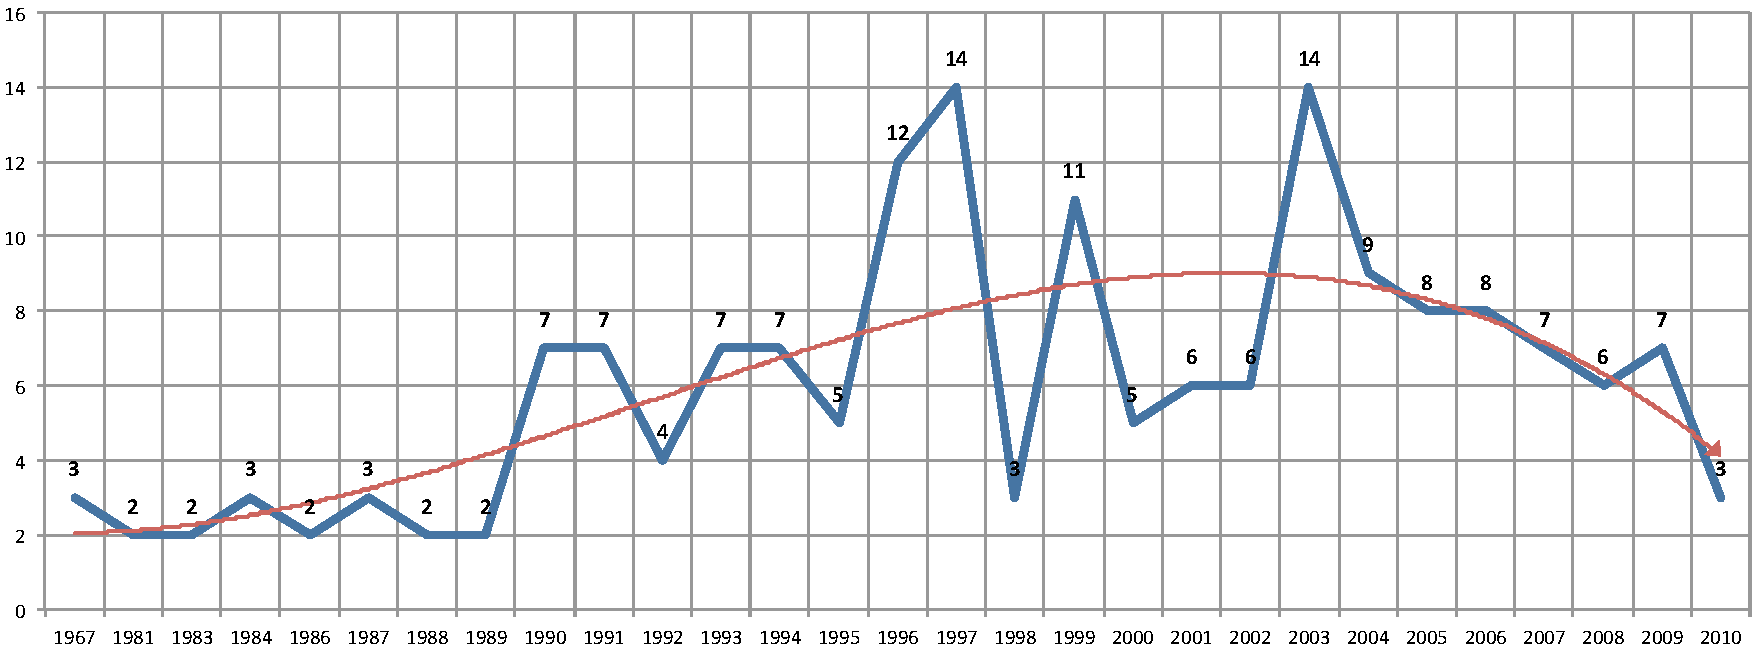
\includegraphics[scale=0.35]{pictures/abntex2-modelo-img-grafico.pdf}
    \end{center}
    \fonte{\textcite[p. 24]{araujo2012} -- \showfont}
\end{figure}

% ---
\subsection{Figuras em minipages}
% ---

Minipages são usadas para inserir textos ou outros elementos em quadros
com tamanhos e posições controladas. Veja o exemplo da
\autoref{fig_minipage_imagem1} e da \autoref{fig_minipage_grafico2} -- \showfont.

\begin{figure}[htb]
\label{teste}
\centering
 \begin{minipage}{0.49\textwidth}
   \caption[Imagem 1 da minipage]{Imagem 1 da minipage -- \showfont}
   \label{fig_minipage_imagem1}
   \centering
   
\includegraphics[width=\textwidth]{pictures/abntex2-modelo-img-marca.pdf}
   \fonte{Produzido pelos autores -- \showfont}
 \end{minipage}
 \hfill
 \begin{minipage}{0.49\textwidth}
   \caption[Gráfico 2 da minipage]{Gráfico 2 da minipage -- \showfont}
   \label{fig_minipage_grafico2}
   \centering
   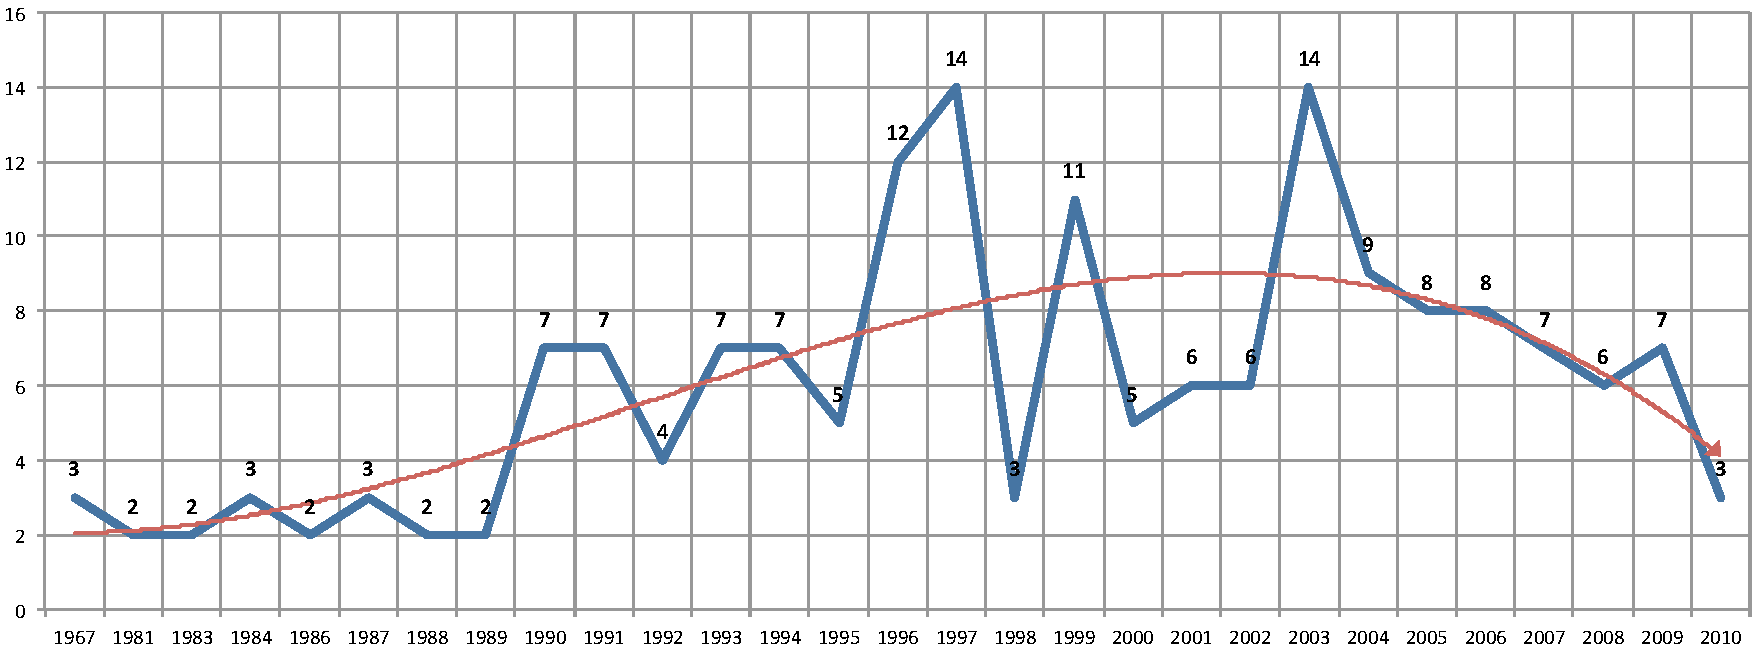
\includegraphics[width=\textwidth]{pictures/abntex2-modelo-img-grafico.pdf}
   \fonte{\textcite[p. 24]{araujo2012} -- \showfont}
 \end{minipage}
\end{figure}



Observe que, segundo a \textcite[seções 4.2.1.10 e 5.8]{NBR14724:2011}, as
ilustrações devem sempre ter numeração contínua e única em todo o documento:

\begin{citacao}
Qualquer que seja o tipo de ilustração, sua identificação aparece na parte
superior, precedida da palavra designativa (desenho, esquema, fluxograma,
fotografia, gráfico, mapa, organograma, planta, quadro, retrato, figura,
imagem, entre outros), seguida de seu número de ordem de ocorrência no texto,
em algarismos arábicos, travessão e do respectivo título. Após a ilustração, na
parte inferior, indicar a fonte consultada (elemento obrigatório, mesmo que
seja produção do próprio autor), legenda, notas e outras informações
necessárias à sua compreensão (se houver). A ilustração deve ser citada no
texto e inserida o mais próximo possível do trecho a que se
refere. \cite[seções 5.8]{NBR14724:2011} -- \showfont
\end{citacao}

% ---
\section{Quadros}
% ---

Depois de definir o ambiente \texttt{quadro} podemos ter um quadro -- \showfont:

\begin{quadro}
\caption[Legenda do primeiro quadro.]{Legenda do primeiro quadro. -- \showfont}
\label{quad:quadro_modelo1}
\centering
\begin{tabular}{|c|}
\hline
Este é o conteúdo do primeiro quadro.\\
\hline
\end{tabular}
\fonte{Teste. -- \showfont}
\end{quadro}


Além do \autoref{quad:quadro_modelo1}, também é possível especificar outra ordem de posicionamento como [htb] -- \showfont:

\begin{quadro}[htb]
\caption[Legenda do segundo quadro.]{Legenda do segundo quadro. -- \showfont}
\label{quad:quadro_modelo2}
\centering
\begin{tabular}{|c|}
\hline
Este é o conteúdo do segundo quadro.\\
\hline
\end{tabular}
\fonte{O autor. -- \showfont}
\end{quadro}



% ---
\section{Expressões matemáticas}
% ---

\index{expressões matemáticas} Use o ambiente \texttt{equation} para escrever
expressões matemáticas numeradas -- \showfont:

\begin{equation}
  \forall x \in X, \quad \exists \: y \leq \epsilon
\end{equation}

Escreva expressões matemáticas entre \$ e \$, como em -- \showfont

 $\lim_{x \to \infty}
\exp(-x) = 0 $, para que fiquem na mesma linha -- \showfont.

Também é possível usar colchetes para indicar o início de uma expressão
matemática que não é numerada -- \showfont.

\[
\left|\sum_{i=1}^n a_ib_i\right|
\le
\left(\sum_{i=1}^n a_i^2\right)^{1/2}
\left(\sum_{i=1}^n b_i^2\right)^{1/2}
\]

Consulte mais informações sobre expressões matemáticas em
\url{https://code.google.com/p/abntex2/wiki/Referencias} -- \showfont.


% ---
\section{Enumerações: alíneas e subalíneas}
% ---

\index{alíneas}\index{subalíneas}\index{incisos}Quando for necessário enumerar
os diversos assuntos de uma seção que não possua título, esta deve ser
subdividida em alíneas -- \showfont \cite[4.2]{NBR6024:2012}:

\begin{alineas}

  \item os diversos assuntos que não possuam título próprio, dentro de uma mesma
  seção, devem ser subdivididos em alíneas -- \showfont;

  \item o texto que antecede as alíneas termina em dois pontos -- \showfont;
  \item as alíneas devem ser indicadas alfabeticamente, em letra minúscula,
  seguida de parêntese. Utilizam-se letras dobradas, quando esgotadas as
  letras do alfabeto;

  \item as letras indicativas das alíneas devem apresentar recuo em relação à
  margem esquerda;

  \item o texto da alínea deve começar por letra minúscula e terminar em
  ponto-e-vírgula, exceto a última alínea que termina em ponto final;

  \item o texto da alínea deve terminar em dois pontos, se houver subalínea;

  \item a segunda e as seguintes linhas do texto da alínea começa sob a
  primeira letra do texto da própria alínea;

  \item subalíneas \cite[4.3]{NBR6024:2012} devem ser conforme as alíneas a
  seguir:

  \begin{alineas}
     \item as subalíneas devem começar por travessão seguido de espaço -- \showfont;

     \item as subalíneas devem apresentar recuo em relação à alínea;

     \item o texto da subalínea deve começar por letra minúscula e terminar em
     ponto-e-vírgula. A última subalínea deve terminar em ponto final, se não
     houver alínea subsequente;

     \item a segunda e as seguintes linhas do texto da subalínea começam sob a
     primeira letra do texto da própria subalínea.
  \end{alineas}

  \item no \abnTeX{} estão disponíveis os ambientes \texttt{incisos} e
  \texttt{subalineas}, que em suma são o mesmo que se criar outro nível de
  \texttt{alineas}, como nos exemplos à seguir:

  \begin{incisos}
    \item \textit{Um novo inciso em itálico} -- \showfont;
  \end{incisos}

  \item Alínea em \textbf{negrito} -- \showfont:

  \begin{subalineas}
    \item \textit{Uma subalínea em itálico};
    \item \underline{\textit{Uma subalínea em itálico e sublinhado}};
  \end{subalineas}

  \item Última alínea com \emph{ênfase}.

\end{alineas}

% ---
\section{Espaçamento entre parágrafos e linhas}
% ---

\index{espaçamento!dos parágrafos}O tamanho do parágrafo, espaço entre a margem
e o início da frase do parágrafo, é definido por:

\begin{lstlisting}[language=tex]
   \setlength{\parindent}{1.3cm}
\end{lstlisting}

\index{espaçamento!do primeiro parágrafo}Por padrão, não há espaçamento no
primeiro parágrafo de cada início de divisão do documento
(\autoref{sec-divisoes}). Porém, você pode definir que o primeiro parágrafo
também seja indentado, como é o caso deste documento. Para isso, apenas inclua o
pacote \textsf{indentfirst} no preâmbulo do documento:

\begin{lstlisting}[language=tex]
   \usepackage{indentfirst}      % Indenta o primeiro parágrafo de cada seção.
\end{lstlisting}

\index{espaçamento!entre os parágrafos}O espaçamento entre um parágrafo e outro
pode ser controlado por meio do comando:

\begin{verbnobox}[\small]
  \setlength{\parskip}{0.2cm}  % tente também \onelineskip
\end{verbnobox}

\index{espaçamento!entre as linhas}O controle do espaçamento entre linhas é
definido por:

\begin{lstlisting}[language=tex]
  \OnehalfSpacing       % espaçamento um e meio (padrão);
  \DoubleSpacing        % espaçamento duplo
  \SingleSpacing        % espaçamento simples
\end{lstlisting}

Para isso, também estão disponíveis os ambientes:

\begin{lstlisting}[language=tex]
  \begin{SingleSpace} ...\end{SingleSpace}
  \begin{Spacing}{hfactori} ... \end{Spacing}
  \begin{OnehalfSpace} ... \end{OnehalfSpace}
  \begin{OnehalfSpace*} ... \end{OnehalfSpace*}
  \begin{DoubleSpace} ... \end{DoubleSpace}
  \begin{DoubleSpace*} ... \end{DoubleSpace*}
\end{lstlisting}

Para mais informações, consulte \textcite[p. 47-52 e 135]{memoir} -- \showfont.

% ---
\section{Inclusão de código fonte}\label{sec-codeinsert}
% ---

\begin{lstlisting}[caption={[Leitura dos dados simulados e conversão para estados topológicos.]{Leitura
    dos dados simulados e conversão para estados topológicos. -- \showfont}},label={lst:leituradadossim}]
% Pré definições iniciais
nsub=3;  % Numero de Submódulos
nbits=2*nsub; % Numero de bits necessários para representar os estados
nlevels=2*nsub+1; % Numero total de níveis

% Leitura dos pontos gerados por simulação
time=data(1,:)'; % extrai vetor de tempo
PWM=logical(data(2:end,:))'; % Conversão dos pulsos PWM para estados lógicos

% Cria vetor de string binário com os estados correspondentes
binstates=num2str([PWM(:,1) PWM(:,3) PWM(:,5) PWM(:,7) PWM(:,9) PWM(:,11)]);
state=fi(bin2dec(binstates),0,nbits,0); % Objeto numérico de ponto-fixo

\end{lstlisting}



\begin{lstlisting}[language=Python,caption={[Python example]{Python example -- \showfont}}]
import numpy as np

def incmatrix(genl1,genl2):
    m = len(genl1)
    n = len(genl2)
    M = None #to become the incidence matrix
    VT = np.zeros((n*m,1), int)  #dummy variable

    #compute the bitwise xor matrix
    M1 = bitxormatrix(genl1)
    M2 = np.triu(bitxormatrix(genl2),1)

    for i in range(m-1):
        for j in range(i+1, m):
            [r,c] = np.where(M2 == M1[i,j])
            for k in range(len(r)):
                VT[(i)*n + r[k]] = 1;
                VT[(i)*n + c[k]] = 1;
                VT[(j)*n + r[k]] = 1;
                VT[(j)*n + c[k]] = 1;

                if M is None:
                    M = np.copy(VT)
                else:
                M = np.concatenate((M, VT), 1)

                VT = np.zeros((n*m,1), int)

    return M
\end{lstlisting}




% ---
\section{Inclusão de outros arquivos}\label{sec-include}
% ---

É uma boa prática dividir o seu documento em diversos arquivos, e não
apenas escrever tudo em um único. Esse recurso foi utilizado neste
documento. Para incluir diferentes arquivos em um arquivo principal,
de modo que cada arquivo incluído fique em uma página diferente, utilize o
comando -- \showfont:

\begin{lstlisting}[language=tex]
   \include{documento-a-ser-incluido}      % sem a extensão .tex
\end{lstlisting}

Para incluir documentos sem quebra de páginas, utilize -- \showfont:

\begin{lstlisting}[language=tex]
   \input{documento-a-ser-incluido}      % sem a extensão .tex
\end{lstlisting}



% ---
\section{Compilar o documento \LaTeX{}}
% ---

Geralmente os editores \LaTeX{}, como o
TeXlipse\footnote{\url{http://texlipse.sourceforge.net/} -- \showfont}, o
Texmaker\footnote{\url{http://www.xm1math.net/texmaker/} -- \showfont}, entre outros,
compilam os documentos automaticamente, de modo que você não precisa se
preocupar com isso -- \showfont.

No entanto, você pode compilar os documentos \LaTeX{} usando os seguintes
comandos, que devem ser digitados no \emph{Prompt de Comandos} do Windows ou no
\emph{Terminal} do Mac ou do Linux -- \showfont:

\begin{lstlisting}[language=bash,caption={[Você pode compilar os documentos \LaTeX{} usando os seguintes
        comandos.]{Você pode compilar os documentos \LaTeX{} usando os seguintes
        comandos. -- \showfont}},label={lst:compilarLatex}]
   pdflatex ARQUIVO_PRINCIPAL.tex
   bibtex ARQUIVO_PRINCIPAL.aux
   makeindex ARQUIVO_PRINCIPAL.idx
   makeindex ARQUIVO_PRINCIPAL.nlo -s nomencl.ist -o
     ARQUIVO_PRINCIPAL.nls
   pdflatex ARQUIVO_PRINCIPAL.tex
   pdflatex ARQUIVO_PRINCIPAL.tex
\end{lstlisting}

\begin{lstlisting}[language=bash]
a very long and totruous path which you can check to see if it breaks and where at the end of the line
\end{lstlisting}



% ---
\section{Remissões internas}
% ---

Ao nomear a \autoref{tab-nivinv} e a \autoref{fig_circulo}, apresentamos um
exemplo de remissão interna, que também pode ser feita quando indicamos o
\autoref{cap_exemplos}, que tem o nome \emph{\nameref{cap_exemplos}}. O número
do capítulo indicado é \ref{cap_exemplos}, que se inicia à
\autopageref{cap_exemplos}\footnote{O número da página de uma remissão pode ser
obtida também assim:
\pageref{cap_exemplos}. -- \showfont}.
Veja a \autoref{sec-divisoes} para outros exemplos de remissões internas entre
seções, subseções e subsubseções.

O código usado para produzir o texto desta seção é -- \showfont:

\begin{lstlisting}[language=TeX,caption={[TeX example]{TeX example -- \showfont}}]
Ao nomear a \autoref{tab-nivinv} e a \autoref{fig_circulo}, apresentamos um
exemplo de remissão interna, que também pode ser feita quando indicamos o
\autoref{cap_exemplos}, que tem o nome \emph{\nameref{cap_exemplos}}. O número
do capítulo indicado é \ref{cap_exemplos}, que se inicia à
\autopageref{cap_exemplos}\footnote{O número da página de uma remissão pode ser
obtida também assim:
\pageref{cap_exemplos}. -- \showfont}.
Veja a \autoref{sec-divisoes} para outros exemplos de remissões internas entre
seções, subseções e subsubseções.
\end{lstlisting}



% ---
\section{Divisões do documento: seção}\label{sec-divisoes}
% ---

Esta seção testa o uso de divisões de documentos. Esta é a
\autoref{sec-divisoes}. Veja a \autoref{sec-divisoes-subsection} -- \showfont.



\subsection{Divisões do documento: subseção}\label{sec-divisoes-subsection}

Isto é uma subseção. Veja a \autoref{sec-divisoes-subsubsection}, que é uma
\texttt{subsubsection  } do \LaTeX{}, mas é impressa chamada de ``subseção'' porque
no Português não temos a palavra ``subsubseção'' -- \showfont.



\subsubsection{Divisões do documento: subsubseção}
\label{sec-divisoes-subsubsection}

Isto é uma subsubseção -- \showfont.



\subsubsection{Divisões do documento: subsubseção}

Isto é outra subsubseção -- \showfont.



\subsection{Divisões do documento: subseção}\label{sec-exemplo-subsec}

Isto é uma subseção -- \showfont.



% ---
\section[Exemplo muito longo]{Este é um exemplo de nome de seção longo. Ele deve estar
alinhado à esquerda e a segunda e demais linhas devem iniciar logo abaixo da
primeira palavra da primeira linha -- \showfont}
% ---

Isso atende à norma \textcite[seções de 5.2.2 a 5.2.4]{NBR14724:2011}
 e \textcite[seções de 3.1 a 3.8]{NBR6024:2012}.



% ---
\section{Diferentes idiomas e hifenizações}
\label{sec-hifenizacao}
% ---

Para usar hifenizações de diferentes idiomas, inclua nas opções do documento o
nome dos idiomas que o seu texto contém. Por exemplo (para melhor
visualização, as opções foram quebras em diferentes linhas) -- \showfont:

\begin{verbnobox}[\small]
\documentclass[
12pt, % Tamanho da fonte
a5paper, % Tamanho do papel
twoside, % Impressão nos dois lados da folha
english,
brazil,
%sumario=tradicional,
%sumario=abnt-6027-2012, % memoir v3.6k ou superior
sumario=UFSC,
chapter=TITLE, % Título de capítulos em caixa alta
section=TITLE  % Título de seções em caixa alta
]{ufsc-inep-thesis}
\end{verbnobox}

O idioma português-brasileiro (\texttt{brazil}) é incluído automaticamente pela
classe \textsf{abntex2}. Porém, mesmo assim a opção \texttt{brazil} deve ser
informada como a última opção da classe para que todos os pacotes reconheçam o
idioma. Vale ressaltar que a última opção de idioma é a utilizada por padrão no
documento. Desse modo, caso deseje escrever um texto em inglês que tenha
citações em português e em francês, você deveria usar o preâmbulo como abaixo -- \showfont:

\begin{verbatim}
\documentclass[
    12pt,
    openright,
    twoside,
    a5paper,
    french,
    brazil,
    english
    ]{ufsc-inep-thesis}
\end{verbatim}

A lista completa de idiomas suportados, bem como outras opções de hifenização,
estão disponíveis em \textcite[p.~5-6]{babel}.

Exemplo de hifenização em inglês\footnote{Extraído de:
\url{http://en.wikibooks.org/wiki/LaTeX/Internationalization} -- \showfont}:

% https://tex.stackexchange.com/questions/20987/changing-babel-package-inside-a-single-chapter
\begin{otherlanguage*}{english}
\textit{Text in English language. This environment switches all language\hyp{}definitions,
like the language specific names for figures, tables etc. to the other
language. The starred version of this environment typesets the main text
according to the rules of the other language, but keeps the language specific
string for ancillary things like figures, in the main language of the document.
The environment hyphenrules switches only the hyphenation patterns used; it can
also be used to disallow hyphenation by using the language name
`nohyphenation'. -- \showfont}
\end{otherlanguage*}

Exemplo de hifenização em francês\footnote{Extraído de:
\url{http://bigbrowser.blog.lemonde.fr/2013/02/17/tu-ne-tweeteras-point-le-vatican-interdit-aux-cardinaux-de-tweeter-pendant-le-conclave/} -- \showfont}:

% https://tex.stackexchange.com/questions/20987/changing-babel-package-inside-a-single-chapter
\begin{otherlanguage*}{french}
\textit{Texte en français. Pas question que Twitter ne vienne faire une
concurrence déloyale à la traditionnelle fumée blanche qui mar\-que l'élection
d'un nouveau pape. Pour éviter toute fuite précoce, le Vatican a donc pris un
peu d'avance, et a déjà interdit aux cardinaux qui prendront part au vote
d'utiliser le réseau social, selon Catholic News Service. Une mesure valable
surtout pour les neuf cardinaux – sur les 117 du conclave – pratiquants très
actifs de Twitter, qui auront interdiction pendant toute la période de se
connecter à leur compte. -- \showfont}
\end{otherlanguage*}

Pequeno texto em espanhol\footnote{Extraído de:
\url{http://internacional.elpais.com/internacional/2013/02/17/actualidad/1361102009_913423.html} -- \showfont}:

\foreignlanguage{spanish}{\textit{Decenas de miles de personas ovacionan al pontífice en su
penúltimo ángelus dominical, el primero desde que anunciase su renuncia. El Papa se
centra en la crítica al materialismo}} -- \showfont.

O idioma geral do texto por ser alterado como no exemplo seguinte -- \showfont:

\begin{verbatim}
  \selectlanguage{english}
\end{verbatim}

Isso altera automaticamente a hifenização e todos os nomes constantes de
referências do documento para o idioma inglês. Consulte o manual da classe
\cite{abntex2classe} para obter orientações adicionais sobre internacionalização de
documentos produzidos com \abnTeX{} -- \showfont.

A \autoref{sec-citacao} descreve o ambiente \texttt{citacao} que pode receber
como parâmetro um idioma a ser usado na citação -- \showfont.



% ---
\section{Consulte o manual da classe \textsf{abntex2}}
% ---

Consulte o manual da classe \textsf{abntex2} \cite{abntex2classe} para uma
referência completa das macros e ambientes disponíveis -- \showfont.

Além disso, o manual possui informações adicionais sobre as normas ABNT
observadas pelo \abnTeX{} e considerações sobre eventuais requisitos específicos
não atendidos, como o caso da \textcite[seção 5.2.2]{NBR14724:2011}, que
especifica o espaçamento entre os capítulos e o início do texto, regra
propositalmente não atendida pelo presente modelo -- \showfont.



% ---
\section{Referências bibliográficas}
% ---

A formatação das referências bibliográficas conforme as regras da ABNT são um
dos principais objetivos do \abnTeX{}. Consulte os manuais
\textcite{abntex2cite} e \textcite{abntex2cite-alf} para obter informações
sobre como utilizar as referências bibliográficas -- \showfont.



%-
\subsection{Acentuação de referências bibliográficas}
%-

Normalmente não há problemas em usar caracteres acentuados em arquivos
bibliográficos (\texttt{*.bib}). Porém, como as regras da ABNT fazem uso quase
abusivo da conversão para letras maiúsculas, é preciso observar o modo como se
escreve os nomes dos autores. Na ~\autoref{tabela-acentos} você encontra alguns
exemplos das conversões mais importantes. Preste atenção especial para `ç' e `í'
que devem estar envoltos em chaves. A regra geral é sempre usar a acentuação
neste modo quando houver conversão para letras maiúsculas -- \showfont.

\begin{table}[htbp]
\caption[Tabela de conversão de acentuação]{Tabela de conversão de acentuação. -- \showfont}
\label{tabela-acentos}
\centering
\begin{tabular}{ll}\hline\hline
acento & \textsf{bibtex}\\
à á ã & \verb+\`a+ \verb+\'a+ \verb+\~a+\\
í & \verb+{\'\i}+\\
ç & \verb+{\c c}+\\
\hline\hline
\end{tabular}
\fonte{Manual do LaTeX \cite{memoir} -- \showfont}
\end{table}



% ---
\section{Precisa de ajuda?}
% ---

Consulte a FAQ com perguntas frequentes e comuns no portal do \abnTeX{}:
\url{https://code.google.com/p/abntex2/wiki/FAQ}.

Inscreva-se no grupo de usuários \LaTeX{}:
\url{http://groups.google.com/group/latex-br}, tire suas dúvidas e ajude
outros usuários.

Participe também do grupo de desenvolvedores do \abnTeX{}:
\url{http://groups.google.com/group/abntex2} e faça sua contribuição à
ferramenta.



% ---
\section{Você pode ajudar?}
% ---

Sua contribuição é muito importante! Você pode ajudar na divulgação, no
desenvolvimento e de várias outras formas. Veja como contribuir com o \abnTeX{}
em \url{https://code.google.com/p/abntex2/wiki/ComoContribuir}.



% https://tex.stackexchange.com/questions/264586/invisible-overfull-hbox-in-toc
% https://tex.stackexchange.com/questions/53513/hyperref-token-not-allowed
\section{Quer customizar os modelos do \texorpdfstring{\newline}{}\abnTeX{} para sua instituição ou
universidade?}

Veja como customizar o \abnTeX{} em:
\url{https://code.google.com/p/abntex2/wiki/ComoCustomizar}.

